\underline{Transformata Fouriera} - badanie sygnału stacjonarnego w dziedzinie częstotliwości.

$ FT(f) = \int_{-\infty}^{\infty} x(t) \cdot e^{-2i\pi f t} dt $

Jeśli wynik tego całkowania ma dużą wartość w punkcie $ f $ oznacz to, że sygnał ma wysoką wartość składowej widmowej o częstości $ f $. W przeciwnym wypadku widmo sygnału nie posida istotnej składowej o tej częstośći.

\underline{Transformata Fouriera w oknie czasowym STFT} - stała się alternatywą dla
transformacji Fouriera z tego względu, że 
nadaje się do analizowania sygnałów niestacjonarnych. Niestacjonarny sygnał dzieli się na okna czasowe, w których powstałe sygnały są w przybliżeniu stacjonarne. Okno czasowe powstają poprzez iloczyn sygnału oraz okna reprezentowanego przez prostokąt ($ f_O = 1 $ w oknie, $ f_O = 0 $ poza oknem). Stosując szerokie okno otrzymujemy dokładne informacje o niskich częstotliwościach, natomiast stosując wąskie okno – dokładne informacje o wysokich częstotliwościach. Wymiary analizowanego okna zmieniają się w zależności od tego, którą
z informacji (o czasie, czy o częstotliwości), chcemy uzyskać z większą
wiarygodnością.

$ STFT(f)_{f_O} = \int_{-\infty}^{\infty} f_O(t_1, t_2) x(t) \cdot e^{-2i\pi f t} dt $

\underline{Ciągła transformata falkowa CWT} - nie zatraca charakteru badanego szeregu, polega na dzieleniu sygnału na mniejsze części, za
pomocą okien wagowych o zmieniających się wymiarach, a następnie na analizowaniu
każdej z nich poprzez porównywanie z przesuniętą i przeskalowaną funkcją podstawową. W wyniku zastosowania CWT otrzymujemy macierz współczynników
mówiących o tym, w jakim stopniu dana część sygnału pokrywa się z porównywaną falką podstawową (rys.~\ref{wavelets}).

\begin{figure} [H]
	\centering
	\begin{subfigure}{.48\textwidth}
		\centering
		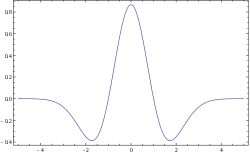
\includegraphics[width=1.0\linewidth]{EDMIIssues/Figures/sombrero.png}
	\end{subfigure}
	\begin{subfigure}{.48\textwidth}
		\centering
		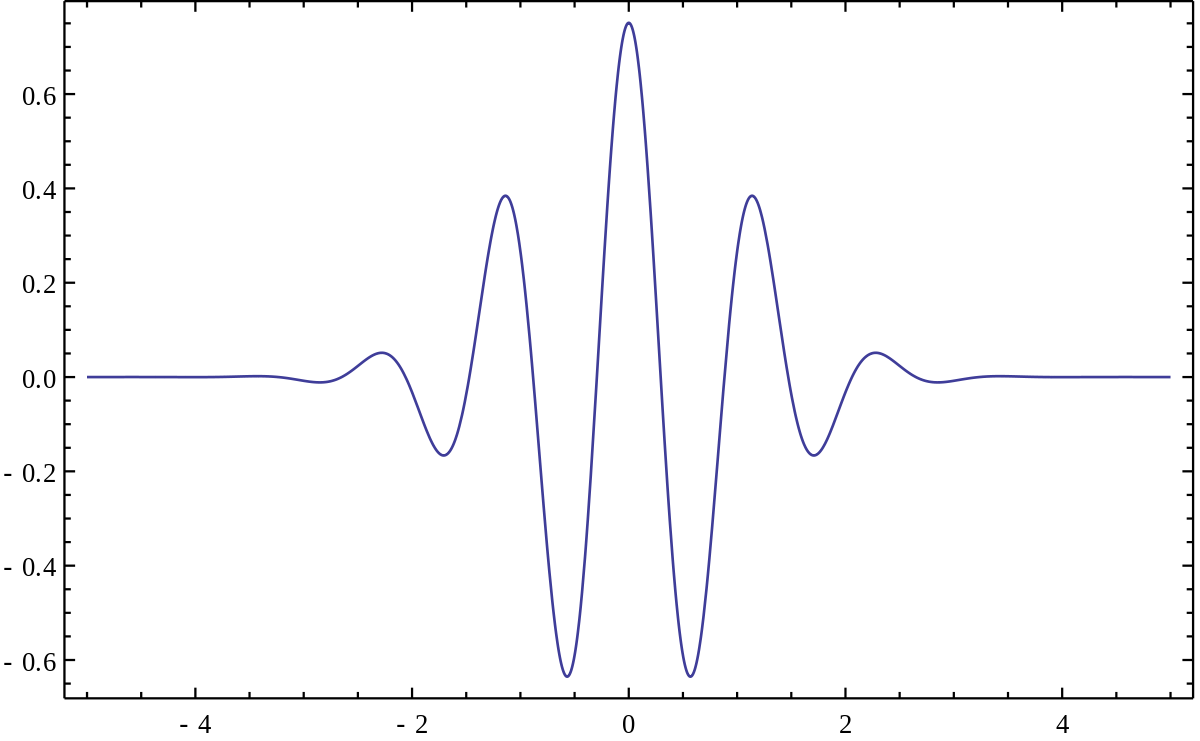
\includegraphics[width=1.0\linewidth]{EDMIIssues/Figures/morlet.png}
	\end{subfigure}
	\caption{Przykładowe falki, po lewej - \textit{sobrero}, po prawej - \textit{morlet}.}
	\label{wavelets}
\end{figure}

$ C(skala, pozycja) = \int f(t) \Psi(skala, pozycja, t) dt $, gdzie: \newline
$ C $ - macierz współczynników, \newline
$ f(t) $ - oryginalny sygnał, \newline
$ \Psi $ - falka.

Dobór skali odbywa się na zasadzie kostki Heisenberga - rozdzielczości czasowa oraz częstościowa zmieniają się, natomiast ich stosunek jest stały.

Ciągła transformacja falkowa zdefiniowana jest jako suma całego omawianego sygnału
pomnożonego przez przeskalowane i przesunięte wersje falki podstawowej:

$ CWT_x^{\Psi^*} (s, \tau) = \int_{-\infty}^{\infty} x(t) \Psi^*_{s, \tau} dt $, gdzie: \newline
$ s $ - skala, \newline
$ \tau $ - przesunięcie (pozycja), \newline
$ x(t) $ - oryginalny sygnał, \newline
$ \Psi^* $ - falka przeskalowana i przesunięta.

$ \Psi^*(s, \tau) = \dfrac{1}{\sqrt{|s|}} \Psi(\dfrac{t- \tau}{s}) $

\underline{Empiryczna analiza modów - EMD}

Funkcja modów własnych spełnia dwa warunki:
\begin{itemize}
	\item Na całej szerokości sygnału liczba przejść przez zero oraz liczba ekstremów musi być, albo jednakowa, albo różnić się maksymalnie o jeden.
	\item W każdym punkcie sygnału średnia wartość obwiedni dolnej oraz górnej wynosi zero.
\end{itemize}

Dekompozycja na mody empiryczne oparta jest na założeniach:\newline
\begin{itemize}
	\item Badany sygnał posiada przynajmniej dwa ekstrema - jedno minimum oraz jedno maksimum.
	\item Charakterystyczna dla sygnału skala czasowa wynika z odstępu między ekstremami.
	\item Jeśli sygnał nie ma żadnych ekstremów, a jedynie punkty przecięcia, można go zróżniczkować jednokrotnie lub wielokrotnie.
\end{itemize}

Procedura "przesiewania" (otrzymywania funckji IMF - \textit{intrinsic mode functions} ) dla metody EMD (rys~\ref{emd}):
\begin{itemize}
	\item Wyznaczyć wszystkie ekstrema sygnału.
	\item Połączyć wszystkie maksyma za pomocą \textit{spline lines} - otrzymujemy obwiednię $ max_i $
	\item To samo dla minimów - otrzymujemy obwiednię $ min_i $
	\item obliczamy średnią $ m_i = \dfrac{min_i + max_i}{2} $
	\item $ h_i = h_{i-1} - m_i $, gdzie $ h_0 = X(t) $. Jeśli w kroku $ i $ prawdziwym będzie kryterium stop np. $ std(h_i, h_{i-1}) < \epsilon $ wtedy nasze $ h_i $ jest modem IMF.
\end{itemize}

\begin{figure} [H]
	\centering
	\begin{subfigure}{.48\textwidth}
		\centering
		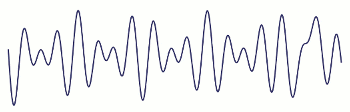
\includegraphics[width=1.0\linewidth]{EDMIIssues/Figures/emd1.png}
	\end{subfigure}
	\begin{subfigure}{.48\textwidth}
		\centering
		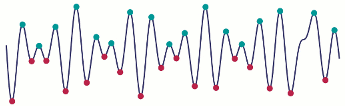
\includegraphics[width=1.0\linewidth]{EDMIIssues/Figures/emd2.png}
	\end{subfigure}
	\begin{subfigure}{.48\textwidth}
		\centering
		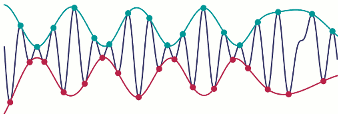
\includegraphics[width=1.0\linewidth]{EDMIIssues/Figures/emd3.png}
	\end{subfigure}
	\begin{subfigure}{.48\textwidth}
		\centering
		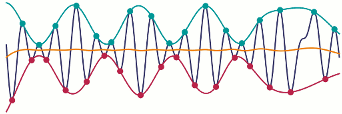
\includegraphics[width=1.0\linewidth]{EDMIIssues/Figures/emd4.png}
	\end{subfigure}
	\caption{Kolejne kroki pojedynczej iteracji procedury "przesiewania" dla metody EMD.}
	\label{emd}
\end{figure}

Kolejne mody otrzymujemy poprzez metode przesiewania dla różnicy sygnału oraz znalezionych modów $ r_{k} = X(t) - \sum_{i=0}^{k} c_i $, gdzie $ k $ - liczba znalezionych modów. Jeśli $ r_k $ jest funckją monotoniczną, więcej modów nie może być znalezione - kończymy procedurę.

EMD może być wykorzystywana np. do badania wad osi układów mechanicznych.